\section{Monitoring Algorithm} 
\label{sec:algorithm}

\bgroup \color{red}
In this section, we give algorithms to compute the STL$^+$ semantics in two different settings: the \emph{offline} setting where the entire execution trace is available at once (\cref{sec:offline}) and the \emph{online} setting where the execution trace becomes available incrementally (\cref{sec:online}).
In the offline setting, our algorithm works both for future STL and past STL.
In the online setting, we consider only past STL.
\egroup

\subsection{Offline Algorithm} \label{sec:offline}
In the offline setting, we assume the entire signal is available to the monitor.
We describe an algorithm, given a distributed signal $(S,{\hb})$ and an STL formula $\varphi$, to compute $[(S,{\hb}) \models \varphi]_+$ using the function $\gamma$ from \cref{sec:approach} without explicitly computing $\tr^+(S,{\hb})$.
We introduce the \emph{asynchronous product} of value expressions to capture interleavings within segments, then evaluate \emph{untimed} and \emph{timed operators}.
Finally, we combine these steps to compute the \emph{semantics} of STL$^+$.

We also discuss an efficient implementation of the monitoring algorithm using \emph{bit vectors}, heuristics to enhance \emph{generalization} for real-valued signals, and a method to \emph{combine} our approach with exact monitoring.

\paragraph*{Asynchronous Products.}
Consider the value expressions $u_1 = 0 \cdot 1$ and $u_2 = 1 \cdot 0$ encoding the behaviors of two signals within a segment.
Since behaviors within a segment are asynchronous, to capture their potential interleavings, we consider how the values in $u_1$ and $u_2$ can align.
In particular, there are three potential alignments:
(i) the rising edge of $u_1$ happens before the falling edge of $u_2$,
(ii) the falling edge of $u_2$ happens before the rising edge of $u_1$, and
(iii) they happen simultaneously.
We respectively represent these with the tuples $(011, 110)$, $(001, 100)$, and $(01, 10)$ where the first component encodes $u_1$ and the second $u_2$.
Formally, given two value expressions $u_1$ and $u_2$ (resp.  sets $L_1$ and $L_2$ of value expressions), we define their \emph{asynchronous product} as follows:

\begin{align*}
	u_1 \otimes u_2 &=
	\begin{aligned}[t]
	\big\{ \destutter(v_1, v_2) \st v_i \in \stutter_k(u_i), \\
		k = |u_1| + |u_2| - 1, i \in \{1,2\} \big\}
	\end{aligned}\\
	L_1 \otimes L_2 &= \{ u_1 \otimes u_2 \st u_1 \in L_1, u_2 \in L_2 \}
\end{align*}

Asynchronous products of value expressions allow us to lift value expressions to satisfaction signals of formulas.

\begin{example} \label{ex:asyncprod}
	Recall $(S, {\hb})$ and its $\gamma$ function given in \cref{fig:csve}.
	To compute the value expressions encoding the satisfaction of $x_1 \land x_2$ in the segment $[1,3)$, we first compute the asynchronous product $\gamma(x_1, [3,4)) \otimes \gamma(x_2, [3,4))$, and then the bitwise conjunction of each pair in the set.
	For example, taking the expression $0  1  0$ for $x_1$ and $0  1$ for $x_2$, the product contains the pair $(010, 011)$.
	Its bitwise conjunction is $0  1  0$, encoding a potential behavior for the satisfaction of $x_1 \land x_2$.
\end{example}

\paragraph*{Untimed Operations.}
As hinted in \cref{ex:asyncprod}, to compute the semantics, we apply bitwise operations on value expressions and their asynchronous products to transform them into encodings of satisfaction signals of formulas.
For example, to determine $[(S, {\hb}) \models \LTLeventually (x_1 \land x_2)]_+$, we first compute for each segment in $G_S$ the set of value expressions for the satisfaction of $x_1 \land x_2$, and then from these compute those of $\LTLeventually (x_1 \land x_2)$.
This compositional approach allows us to evaluate arbitrary STL$^+$ formulas.

\bgroup \color{red}
First, we define bitwise operations on Boolean value expressions encoding atomic propositions.
Then, we use these to evaluate untimed STL formulas over sets of value expressions.
Let $u$ and $v$ be Boolean value expressions of length $\ell$.
We denote by $u \BitAnd v$ the bitwise-and operation, by $u \BitOr v$ the bitwise-or, and by $\BitNeg u$ the bitwise-negation.
We also define the \emph{bitwise strong until} and \emph{bitwise strong since} operators:
\begin{align*}
	u \mathsf{U}^0 v &= \left( \max_{i \leq j \leq \ell} \left( \min \left( v[j], \min_{i \leq k \leq j} u[k] \right) \right) \right)_{1 \leq i \leq \ell} \\
	u \mathsf{S}^0 v &= \left( \max_{1 \leq j \leq i} \left( \min \left( v[j], \min_{j \leq k \leq i} u[k] \right) \right) \right)_{1 \leq i \leq \ell}
\end{align*}
As usual, we derive \emph{bitwise eventually} as 
$\mathsf{E} u = 1^\ell \mathsf{U}^0 u$, \emph{bitwise always} as $\mathsf{A} u = \BitNeg 
(\mathsf{E} \BitNeg u)$, and \emph{bitwise weak until} as $u \mathsf{U}^1 v = (u \mathsf{U}^0 v) 
\BitOr (\mathsf{A} u)$.
The corresponding past-time operations are defined similarly:
$\bar{\mathsf{E}} u = 1^\ell \mathsf{S}^0 u$,
$\bar{\mathsf{A}} u = \BitNeg (\bar{\mathsf{E}} \BitNeg u)$, and 
$u \mathsf{S}^1 v = (u \mathsf{S}^0 v) \BitOr (\bar{\mathsf{A}} u)$.
The distinction between $\mathsf{U}^0$ and $\mathsf{U}^1$ (resp. $\mathsf{S}^0$ and $\mathsf{S}^1$) will be useful when we incrementally evaluate a formula.
Finally, note that the output of these operations is a value expression of length $\ell$.
For example, if $u = 010$, we have $\mathsf{E} u = 110$ and $\mathsf{A} u = 000$.
\egroup

Let  $(S, {\hb})$ be a distributed signal.
Consider an atomic proposition $p \in \AP$ encoded as $x_p \in S$ and let $\varphi_1, \varphi_2$ be two STL formulas.
We define the evaluation of untimed formulas with respect to $(S, {\hb})$ and a segment $I \in G_S$ inductively as shown in \cref{fig:eval}.
When $\varphi$ is a future (resp. past) formula and $I$ is the first (resp. last) segment in $G_S$, we simply write $\llbracket (S, {\hb}) \models \varphi \rrbracket$.

\begin{figure*}[!t]
	\begin{align*}
		\llbracket (S, {\hb}), I \models p \rrbracket &= \gamma(x_p, I) \\
		\llbracket (S, {\hb}), I \models \lnot \varphi_1 \rrbracket &= \{\BitNeg u \st u \in  \llbracket (S, {\hb}), I \models \varphi_1 \rrbracket \} \\
		\llbracket (S, {\hb}), I \models \varphi_1 \land \varphi_2 \rrbracket &= \destutter(\{ u_1 \BitAnd u_2 \st (u_1, u_2) \in \llbracket (S, {\hb}), I \models \varphi_1 \rrbracket \otimes \llbracket (S, {\hb}), I \models \varphi_2 \rrbracket  \}) \\
		\llbracket (S, {\hb}), I \models \varphi_1 \until \varphi_2 \rrbracket &= \destutter(\{ u_1 \mathsf{U}^a u_2 \st (u_1, u_2) \in \llbracket (S, {\hb}), I \models \varphi_1 \rrbracket \otimes \llbracket (S, {\hb}), I \models \varphi_2 \rrbracket, \\
		&\hspace{17em} a \in \first(\llbracket (S, {\hb}), I' \models \varphi_1 \until \varphi_2 \rrbracket) \}) \\
		\bgroup \color{red}\llbracket (S, {\hb}), I \models \varphi_1 \since \varphi_2 \rrbracket \egroup &= \destutter(\{ u_1 \mathsf{S}^a u_2 \st (u_1, u_2) \in \llbracket (S, {\hb}), I \models \varphi_1 \rrbracket \otimes \llbracket (S, {\hb}), I \models \varphi_2 \rrbracket, \\
		&\hspace{17em} a \in \last(\llbracket (S, {\hb}), I'' \models \varphi_1 \since \varphi_2 \rrbracket) \})
	\end{align*}
	\caption{Inductive evaluation of untimed formulas, where $I'$ is the segment that follows $I$ in $G_S$  and  $I''$ is the segment that precedes $I$ in $G_S$ (if such segments exist). For completeness, for every formula $\varphi$ we define $\llbracket (S, {\hb}), J \models \varphi \rrbracket = \{0\}$ when $J \notin G_S$. \label{fig:eval}}
\end{figure*}

Similarly as above, we can use the standard derived operators to compute the corresponding sets of value expressions.
For a given formula and a segment, the evaluation above produces a set of value expressions encoding the formula's satisfaction within the segment.

\begin{example}
	Recall $(S, {\hb})$ and $\gamma$ from \cref{fig:csve}.
	To compute $\llbracket (S, {\hb}), [5,7) \models \LTLeventually(x_1 \land x_2) \rrbracket$, we first compute $\llbracket (S, {\hb}), [5,7) \models x_1 \land x_2 \rrbracket$ by taking the bitwise conjunction over the asynchronous product $\gamma(x_1, [5,7)) \otimes \gamma(x_2, [5,7))$ and destuttering.
	For example, since $010 \in \gamma(x_1, [5,7))$ and $01 \in \gamma(x_2, [5,7))$, the pair $(0010,0111)$ is in the product, whose conjunction gives us $010$ after destuttering. 
	Repeating this for the rest, we obtain $\llbracket (S, {\hb}), [5,7) \models x_1 \land x_2 \rrbracket = \{ 0, 01, 010, 1, 10 \}$.
	Finally, we compute $\llbracket (S, {\hb}), [5,7) \models \LTLeventually(x_1 \land x_2) \rrbracket$ by applying each expression in $\llbracket (S, {\hb}), [5,7) \models x_1 \land x_2 \rrbracket$ the bitwise eventually operator and destuttering.
	The resulting set $\{0, 1, 10\}$ encodes the satisfaction signal of $\LTLeventually(x_1 \land x_2)$ in $[5,7)$.
	Note that we do not need to consider the evaluation of the next segment for the eventually operator since $\llbracket (S, {\hb}), [7,8) \models x_1 \land x_2 \rrbracket = \{0\}$.
\end{example}

\paragraph*{Timed Operations.}
Handling timed operations requires a closer inspection as value expressions are untimed by definition.
We address this issue by considering how a given evaluation interval relates with a given segmentation.
For example, take a segmentation $G_S = \{ [0,4), [4,6), [6,10) \}$ and an evaluation interval $J = [0,5)$.
Suppose we are interested in how a signal $x \in S$ behaves with respect to $J$ over the first segment $I = [0,4)$.
First, to see how $J$ relates with $G_S$ with respect to $I =[0,4)$, we  ``slide'' the interval $J$ over $I \oplus J = [0,9)$ and consider the different ways it intersects the segments in $G_S$.
Initially, $J$ covers the entire segment $[0,4)$ and the beginning of $[4,6)$, for which the potential behaviors of $x$ are captured by the set $\gamma(x, [0,4)) \cdot \pfx(\gamma(x, [4,6)))$.
Now, if we slide the window and take $J' = [3,7)$, the window covers the ending of $[0,4)$, the entire $[4,6)$, and the beginning of $[6,10)$, for which the potential behaviors are captured by $\sfx(\gamma(x, [0,4))) \cdot \gamma(x, [4,6)) \cdot \pfx(\gamma(x, [6,9))$.
We call these sets the \emph{forward profiles} of $J$ and $J'$ with respect to $(S,{\hb})$, $x$, and~$I$.
The \emph{backward profiles} are defined similarly, moving the window towards the past instead of the future.

We first present the definitions, and then demonstrate them in \cref{ex:profiles,ex:timed} and \cref{fig:profiles}. 
Let $(S,{\hb})$ be a distributed signal, $I \in G_S$ be a segment, and $\varphi$ be an STL formula.
Let us introduce some notation.
First, we abbreviate the set $\llbracket (S,{\hb}), I \models \varphi \rrbracket$ of value expressions as $\tau_{\varphi,I}$.
Second, given an interval $K$, we respectively denote by $l_K$ and $r_K$ its left and right end points.
Third, recall that we denote by $F$ the set of end points of $G_S$ (see \cref{sec:approach}).
Given an interval $J$, we define the \emph{profile} of $J$ with respect to $(S,{\hb})$, $\varphi$, and 
$I$ as shown in \cref{fig:profilesDefn}a.
We define \emph{forward profiles} and \emph{backward profiles} to formalize the intuitive approach of ``sliding'' $J$ over the segmentation to obtain the various profiles it produces in \cref{fig:profilesDefn}b and \cref{fig:profilesDefn}c.

\begin{figure*}[!t]
	\begin{align*}
		\textbf{(a) }
		\mathsf{profile}((S,{\hb}), \varphi, I, J) =
		\begin{cases}
			\pfx(\tau_{\varphi,I}) & \text{if } l_I = l_J \land r_I > r_J \\
			\infx(\tau_{\varphi,I}) & \text{if } l_I < l_J \land r_I > r_J \\
			\tau_{\varphi,I} \cdot \kappa(\varphi, I, J) & \text{if } l_I = l_J \land r_I \leq r_J \land r_J \in F \setminus J \\
			\tau_{\varphi,I} \cdot \kappa(\varphi, I, J) \cdot \first(\tau_{\varphi,I'}) & \text{if } l_I = l_J \land r_I \leq r_J \land r_J \in F \cap J  \\		
			\tau_{\varphi,I} \cdot \kappa(\varphi, I, J) \cdot \pfx(\tau_{\varphi,I'}) & \text{if } l_I = l_J \land r_I \leq r_J \land r_J \notin F  \\
			\sfx(\tau_{\varphi,I}) \cdot \kappa(\varphi, I, J) & \text{if }  l_I < l_J < r_I \leq r_J \land r_J \in F \setminus J  \\
			\sfx(\tau_{\varphi,I}) \cdot \kappa(\varphi, I, J) \cdot \first(\tau_{\varphi,I'}) & \text{if } l_I < l_J < r_I \leq r_J \land r_J \in F \cap J \\
			\sfx(\tau_{\varphi,I}) \cdot \kappa(\varphi, I, J) \cdot \pfx(\tau_{\varphi,I'}) & \text{if } l_I < l_J < r_I \leq r_J \land r_J \notin F \\
			\{\epsilon\} & \text{otherwise}
		\end{cases}
	\end{align*}
	\begin{align*}
		\textbf{(b) }
		\mathsf{fwPfs}((S,{\hb}), \varphi, I, J) = \{\destutter(\mathsf{profile}((S,{\hb}), \varphi, I, J')) \st J' \subseteq I \oplus J, J' \sim J\}
	\end{align*}
	\begin{align*}
		\textbf{(c) }
		\bgroup \color{red} \mathsf{bwPfs}((S,{\hb}), \varphi, I, J) \egroup = \{\destutter(\mathsf{profile}((S,{\hb}), \varphi, I, J')) \st J' \subseteq I \ominus J, J' \sim J\}
	\end{align*}
	\caption{Key definitions for the evaluation of timed formulas.
		\textbf{(a)}~The \emph{profile} of an interval $J$ (with respect to $(S,{\hb})$, $\varphi$, and $I$).
		We assume $J$ is trimmed to fit the temporal domain of $S$ and $I' \in G_S$ is such that $r_J \in I'$.
		Moreover, $\kappa(\varphi, I, J)$ is the concatenation $\tau_{\varphi,I_1} \cdot \ldots \cdot \tau_{\varphi,I_m}$ such that $I, I_1, \ldots, I_m, I'$ are consecutive segments in $G_S$.
		If $I_1, \ldots, I_m$ do not exist, we let $\kappa(\varphi, I, J) = \{\epsilon\}$.
		Note that the last case happens when $I \cap J$ is empty.
		\textbf{(b)}~The \emph{forward profiles} of an interval $J$, where $J' \sim J$ holds when $|J'| = |J|$ and $J'$ contains an end point (left or right) iff $J$ does so.
		Note that although infinitely many intervals $J'$ satisfy the conditions given above (due to denseness of time), the set defined by $\mathsf{fwPfs}$ is finite.
		\textbf{(c)}~The \emph{backward profiles} of an interval $J$, where the only difference to forward profiles is that the window slides towards the past instead (using $\ominus$ instead of $\oplus$).
		\label{fig:profilesDefn}}
\end{figure*}

While one may obtain infinitely many intervals by sliding a window on another, the sets of forward and backward profiles are finite.
We demonstrate this and the computation of $\mathsf{fwPfs}$ in \cref{ex:profiles} and \cref{fig:profiles}.

\begin{example} \label{ex:profiles}
	Recall $(S, {\hb})$ and $\gamma$ from \cref{fig:csve}.
	We describe the computation of $\mathsf{fwPfs}((S,{\hb}), x_1, [1,3), [0,1))$.
	Sliding the interval $[0,1)$ over the window $[1,3) \oplus [0,1)$ (see \cref{fig:profiles}) gives us the following sets:
	\begin{align*}
		P_1 &= \destutter(\pfx(\gamma(x_1, [1,3)))) \\
		P_2 &= \destutter(\infx(\gamma(x_1, [1,3)))) \\
		P_3 &= \destutter(\sfx(\gamma(x_1, [1,3))))
	\end{align*}
	where all equal to $\{ 0, 01, 1 \}$.
	Moreover, we have
	\begin{multline*}
		P_4 = \destutter(\sfx(\gamma(x_1, [1,3))) \\ \phantom{kkkkk}\cdot \pfx(\gamma(x_1, [3,4)))) \\ = \{ 0, 01, 010, 0101, 01010, 1, 10, 101, 1010 \}
	\end{multline*}
	We obtain that $\mathsf{fwPfs}((S,{\hb}), x_1, [1,3), [0,1)) = \{P_1, P_2, P_3, P_4\}$.
	This set overapproximates the potential behaviors of $x_1$, for all $t \in [1,3)$, in the interval $t \oplus [0,1)$.
\end{example}

Let $\varphi_1$ and $\varphi_2$ be two STL formulas.
Intuitively, once we have the profiles of a given interval $J$ with respect to $\varphi_1$ and $\varphi_2$, we can evaluate the corresponding untimed formulas on the product of these profiles and concatenate them.
This captures the behavior of the satisfaction signals with respect to a bounded interval, but introduces further overapproximation due to additional concatenations.
Formally, we handle the evaluation of timed formulas as shown in \cref{fig:timedEval}.
Let us demonstrate these definitions on an example.

\begin{figure*}[!t]
	\begin{align*}
		\textbf{(a) }
		\llbracket (S, {\hb}), I \models \varphi_1 \until_J \varphi_2 \rrbracket = \destutter( \{ u_1 \mathsf{U}^0 u_2 \st &(u_1, u_2) \in P_1 \otimes Q_1 \} \cdot \ldots \\ 
		&\ldots \cdot \{ u_1 \mathsf{U}^0 u_2 \st (u_1, u_2) \in P_k \otimes Q_k \} )
	\end{align*}
	\begin{align*}
		\textbf{(b) }
		\bgroup \color{red} \llbracket (S, {\hb}), I \models \varphi_1 \since_J \varphi_2 \rrbracket \egroup = \destutter( \{ u_1 \mathsf{S}^0 u_2 \st &(u_1, u_2) \in P_1' \otimes Q_1' \} \cdot \ldots \\ 
		&\ldots \cdot \{ u_1 \mathsf{S}^0 u_2 \st (u_1, u_2) \in P_k' \otimes Q_k' \} )
	\end{align*}
	\caption{Inductive evaluation of timed formulas where $J$ is a bounded interval.
		\textbf{(a)}~Evaluation of timed until, where $\mathsf{fwPfs}((S,{\hb}), \varphi_1, I, J) = \{P_1, \ldots, P_k \}$ and $\mathsf{fwPfs}((S,{\hb}), \varphi_2, I, J) = \{Q_1, \ldots, Q_k \}$ such that the intervals producing $P_i$ and $Q_i$ respectively start before those producing $P_{i+1}$ and $Q_{i+1}$ for all $1 \leq i < k$.
		\textbf{(b)}~Evaluation of timed since, where $\mathsf{bwPfs}((S,{\hb}), \varphi_1, I, J) = \{P_1', \ldots, P_k' \}$ and $\mathsf{bwPfs}((S,{\hb}), \varphi_2, I, J) = \{Q_1', \ldots, Q_k' \}$ such that the intervals producing $P_i$ and $Q_i$ respectively start before those producing $P_{i+1}$ and $Q_{i+1}$ for all $1 \leq i < k$.
		\label{fig:timedEval}}
\end{figure*}

\begin{example} \label{ex:timed}
	Let $(S, {\hb})$ and $\gamma$ be as in \cref{fig:csve}.
	We demonstrate the evaluation of the timed formula $\LTLeventually_{[0,1)} x_1$ over the segment $[1,3)$.
	Recall from \cref{ex:profiles} the set $\mathsf{fwPfs}((S,{\hb}), x_1, [1,3), [0,1)) = \{P_1, P_2, P_3, P_4\}$ of profiles.
	First, we apply the bitwise eventually operator to each value expression in each of these profiles separately:
	\begin{align*}
		P_1' &= \{ \mathsf{E} u \st u \in P_1 \} = \{ 0, 1 \} \\
		P_2' &= \{ \mathsf{E} u \st u \in P_2 \} = \{ 0, 1 \} \\
		P_3' &= \{ \mathsf{E} u \st u \in P_3 \} = \{ 0, 1 \} \\
		P_4' &= \{ \mathsf{E} u \st u \in P_4 \} = \{ 0, 10, 1 \} \\
	\end{align*}
	We then concatenate these and destutter to obtain 
	\begin{multline*}
		\llbracket (S, {\hb}), [1,3) \models \LTLeventually_{[0,1)} x_1 \rrbracket \\= \{ 0, 01, 010, 0101, 01010, 1, 10, 101, 1010 \}. 
	\end{multline*}
\end{example}

\bgroup \color{red}
\begin{remark}
	Consider the formula $\varphi_1 \until_I \varphi_2$ where $\inf I > 0$ and $\sup I = \infty$.
	We can evaluate this formula similarly to its untimed counterpart $\varphi_1 \until \varphi_2$ (\cref{fig:eval}).
	Recall that the untimed one's evaluation looks at the next segment's first bits to determine whether to apply $\mathsf{U}^0$ or $\mathsf{U}^1$.
	For the timed one, we can use the same logic with an additional look-ahead of $\inf I$.
	In particular, if $\inf I$ coincides with a future segment's left end point, we consider that segment's first bits; otherwise $\inf I$ falls strictly in a segment, in which case we consider all possible truth values of $\varphi_1 \until \varphi_2$ in that segment since signals are asynchronous within each segment.
	The same applies to timed since formulas.
\end{remark}
\egroup


\paragraph*{Computing the Semantics of STL$^+$.}

Putting it all together, given a distributed signal $(S, {\hb})$ and an STL$^+$ formula $\varphi$, we can compute $[(S,{\hb}) \models \varphi]_+$ thanks to the following theorem.

\bgroup \color{red}
\begin{theorem} \label{cl:algo}
	Consider a distributed signal $(S,{\hb})$ and an STL formula $\varphi$.
	If $\varphi$ is a future (resp. past) formula, let $f = \first$ (resp. $f = \last$).
	Then, the following equivalences hold:
	\begin{align*}
		[(S,{\hb}) \models \varphi]_+ = \top &\iff f(\llbracket (S, {\hb}) \models \varphi \rrbracket) = \{1\}\\
		[(S,{\hb}) \models \varphi]_+ = \bot &\iff f(\llbracket (S, {\hb}) \models \varphi \rrbracket) = \{0\}\\
		[(S,{\hb}) \models \varphi]_+ = {?} &\iff f(\llbracket (S, {\hb}) \models \varphi \rrbracket) = \{0,1\}
	\end{align*}
\end{theorem}
\egroup

\begin{figure}
	\centering
	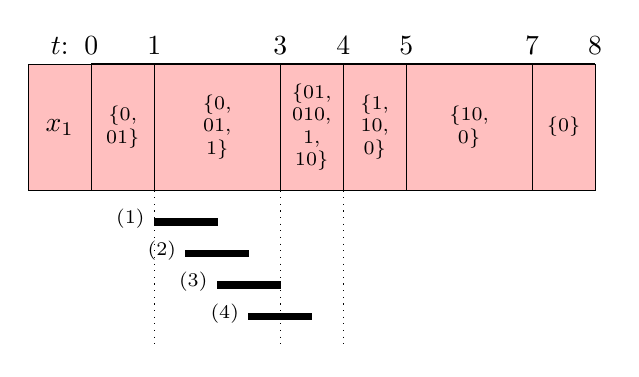
\begin{tikzpicture}[scale=0.8]
		\draw[thick] (0,-5) -- (8,-5);
		\foreach \x in {0,1,3,4,5,7,8}
		\draw (\x,-5) node[above] {\x};
		\draw (-0.5,-5) node[above] {$t$:};
		
		\draw[fill=pink] (-1,-7) rectangle (0,-5) node[midway] {$x_1$};
		\draw[fill=pink] (0,-7) rectangle (1,-5) node[midway] {\scriptsize\begin{tabular}{c}\{0,\\ 01\}\\\end{tabular}};
		\draw[fill=pink] (1,-7) rectangle (3,-5) node[midway] {\scriptsize\begin{tabular}{c}\{0,\\ 01,\\ 1\}\\\end{tabular}};
		\draw[fill=pink] (3,-7) rectangle (4,-5) node[midway] {\scriptsize{\begin{tabular}{c}\{01,\\ 010,\\ 1,\\ 10\}\\\end{tabular}}};
		\draw[fill=pink] (4,-7) rectangle (5,-5) node[midway] {\scriptsize\begin{tabular}{c}\{1,\\ 10,\\ 0\}\\\end{tabular}};
		\draw[fill=pink] (5,-7) rectangle (7,-5) node[midway] {{\scriptsize\begin{tabular}{c}\{10,\\ 0\}\\\end{tabular}}};
		\draw[fill=pink] (7,-7) rectangle (8,-5) node[midway] {{\scriptsize\begin{tabular}{c}\{0\}\\\end{tabular}}};
		
		\draw[dotted] (1,-7) -- (1,-9.5);
		\draw[dotted] (3,-7) -- (3,-9.5);
		\draw[dotted] (4,-7) -- (4,-9.5);
		
		\draw[fill=black] (1, -7.5 + 0.05) node[left]{{\scriptsize (1)}} rectangle (2, -7.5 - 0.05) ;
		\draw[fill=black] (1.5, -8 + 0.05) node[left] {{\scriptsize (2)}} rectangle (2.5, -8 - 0.05) ;
		\draw[fill=black] (2, -8.5 + 0.05) node[left] {{\scriptsize (3)}} rectangle (3, -8.5 - 0.05);
		\draw[fill=black] (2.5, -9 + 0.05) node[left] {{\scriptsize (4)}} rectangle (3.5, -9 - 0.05);
	\end{tikzpicture}
	\caption{Forward profiles of $J = [0,1)$ with respect to $x_1 \in~S$ of \cref{fig:csve}. A representative interval for each profile is shown with solid black lines below the table.}
	\label{fig:profiles}
\end{figure}

\paragraph*{Sets of Boolean Value Expressions as Bit Vectors.}
Asynchronous products are expensive to compute.
Our implementation relies on the observation that sets of boolean value expressions and their operations can be efficiently implemented through bit vectors.
Intuitively, to represent such a set, we encode each element using its first bit and its length since value expressions are boolean and always destuttered.
Moreover, to evaluate untimed operations on such sets, we only need to know the maximal lengths of the four possible types of expressions ($0 \ldots 0$, $0 \ldots 1$, $1 \ldots 0$, and $1 \ldots 1$) and whether the set contains $0$ or $1$ (to handle some edge cases).
This is because value expressions within the same segments are completely asynchronous and the possible interleavings obtained from shorter expressions can be also obtained from longer ones.
%This approach enables, for example, an algorithm for conjunction of sets of value expressions that runs in $O(|u| + |v|)$ time where $u$ and $v$ are the longest expressions in the two sets.
%The same idea also applies to untimed temporal operators.

%\vspace{-0.5em}
\paragraph*{Generalization to Real-Valued Signals.}
Our approximate distributed monitoring method, denoted \textsc{Adm}, can be extended to real-valued signals and numerical predicates.
The key is that finite-length piecewise-constant signals take finitely many values.
By defining $\Sigma$ as a finite alphabet of these values, we can compute atomic propositions as above.
%%Arithmetic operations are handled by computing the asynchronous product of the signals and applying the operation letter-by-letter, transforming the results into atomic propositions via comparison with constants.
For example, if the asynchronous product of two signals $x_1$ and $x_2$ yields $(2\cdot2\cdot3, 1\cdot0\cdot1)$, adding these letter-by-letter results in $3 \cdot 2 \cdot 4$, and comparing with $> 2$ gives $101$.
%%Repeating this for all pairs produces the required atomic proposition.
%\alert{This approach is called \textsc{Orig}.}

We can avoid explicit computation of asynchronous products for some formulas and numerical predicates.
Since signals are asynchronous within segments, we can compute potential value sets instead of sequences.
This approach is called \emph{Fine}, denoted by \textsc{Adm-F}.
Assuming signals are piecewise constant, we can avoid explicit interleaving computations by only considering how potential signal values aggregate.
For instance, with $X_1 = \{2,3\}$ and $X_2 = \{0,1\}$, pairwise addition yields $\{2, 3, 4\}$.
Note that \textsc{Adm-F} overapproximates traces when order matters.
While \textsc{Adm-F} overapproximates traces when order matters, such as in $(x_1 > c_1) \until (x_2 > c_2)$, it preserves precision for formulas like $\LTLalways(x_1 + x_2 > c)$.
The approach \emph{Coarse}, denoted \textsc{Adm-C}, abstracts \emph{Fine} by only considering extreme values, which is useful for monotonic operations where the extreme values of outputs derive from inputs.

We assumed so far that the central monitor runs on a process independent of the observed agents.
Lastly, we also consider a setting where the monitor runs on one of the observed agents.
This approach reduces asynchrony by using the agent's local clock as a reference point for the monitor.
We call this \emph{Relative}, denoted \textsc{Adm-Fr} or \textsc{Adm-Cr} depending on the approach it is paired with.
We evaluate these in \cref{sec:experiments}.

\paragraph*{Combining Exact and Approximate Monitoring.}
We propose a method that combines approximate distributed monitors (\textsc{Adm}) with their exact counterparts (\textsc{Edm}) with the aim to achieve better performance while remaining precise.

The approach works as follows:
Given a distributed signal $(S,{\hb})$ and a formula $\varphi$, compute the approximate verdict $v \gets [(S,{\hb}) \models \varphi]_+$.
If the verdict is inconclusive, i.e., $v = {\,?}$, then compute and return the exact verdict $[(S,{\hb}) \models \varphi]$, else return $v$.
We evaluate this approach in \cref{sec:experiments}.

\bgroup \color{red}
\subsection{Online Algorithm}\label{sec:online}
We now focus on the online setting, where the monitor does not have access to the entire signal, but it periodically reads a new \emph{portion} of the distributed signal $(S,{\hb})$ of a fixed length.
Our goal is to describe an algorithm that computes, given a past STL formula $\varphi$, the value expressions for the satisfaction of $\varphi$ after reading each new signal portion.

Let us first highlight the main difference of the online setting from the offline one.
Unlike in the offline setting, the monitor does not know whether the current signal portion is the last one or not.
After processing consecutive portions of a signal of length $d$, an edge in the next portion with a local timestamp of $t' \in (d, d+\varepsilon)$ may result in new potential interleavings with the edges that have been observed in the current portion.
As a result, if the monitor attempts to produce a verdict for the signal prefix until length $d$, it may produce unsound verdicts as it may miss potential interleavings of edges.
This problem of ``forward uncertainty'' can be avoided if the monitor only produces a verdict for the signal's prefix of length $d-\varepsilon$, since no edge with a local timestamp larger than $d$ can influence the verdict at time $d-\varepsilon$ with respect to the monitor's clock.

Below, we detail two contrasting solutions: a \emph{naive} approach that recomputes everything from scratch after each new portion arrives, and an \emph{incremental} approach that takes advantage of the inductive computation of value expressions.
We demonstrate these in \cref{fig:online}.

\begin{figure*}
	%	\vspace{-1em}
	\centering
		\begin{subfigure}[c]{.1\textwidth}
		\centering
		\begin{tikzpicture}[scale=0.75,>=stealth]
			% portion labels
			\node[anchor=east] at ($(-1,3.6)$) {};
			\vspace{1em}
			\node[anchor=east] at ($(-1,3)$) {\footnotesize{Portion 1}};
			\node[anchor=east] at ($(-1,1.5)$) {\footnotesize{Portion 2}};
			\node[anchor=east] at ($(-1,0)$)       {{\footnotesize Portion 3}};
		\end{tikzpicture}
	\end{subfigure}
%	\hspace{1em}
	\begin{subfigure}[c]{.42\textwidth}
		\centering
		\begin{tikzpicture}[scale=0.75,
			>=stealth,
			box/.style = {fill=gray!40, draw=black, fill opacity=.45}
			]

			%--- handy lengths ------------------------------------------------------------
			\def\DL{2.5}        % 1·Δ  (horizontal unit)
			\def\eps{1.0}      % ε   (shown as small offset of the dashed line)
			\def\del{0.05}      % δ   (horizontal shift used in panel b)
			\def\vsep{1.5}      % vertical separation between rows
			\def\arrowL{3*\DL+0.5}  % total arrow length (both panels)
			\def\barH{0.28}   % <── height of the grey bar
			
			%--- column anchors -----------------------------------------------------------
			\coordinate (A) at (0,0);             % left column (a)
			
			%==============================================================================
			%                               panel (a)
			%------------------------------------------------------------------------------
			\scriptsize
			\node at ($(A)+(1.5*\DL,2.1*\vsep+0.9)$) {\textbf{(a)}};
			\footnotesize
			
			% portion labels
%			\node[anchor=east] at ($(A)+(-0.8,2*\vsep)$) {Portion 1};
%			\node[anchor=east] at ($(A)+(-0.8,1*\vsep)$) {Portion 2};
%			\node[anchor=east] at ($(A)+(-0.8,0)$)       {Portion 3};
			
			% -- row 1 -------------------------------------------------
			\draw[->] ($(A)+(0.5,2*\vsep)$) -- ++(\arrowL,0);
			\path ($(A)+(0.5,2*\vsep)$) coordinate (s1a);
			\filldraw[box] ($(s1a)+(0,-\barH/2)$) rectangle ++(\DL,\barH);
			\draw[solid] ($(s1a)+(0,0.4)$) -- ++(0,-0.8);
			\draw[solid] ($(s1a)+(\DL,0.4)$) -- ++(0,-0.8);
			\draw[dashed] ($(s1a)+(\DL-\eps,0.4)$) -- ++(0,-0.8);
			\node[below]  at ($(s1a)+(0,     -0.4)$) {$0$};
			\node[below]  at ($(s1a)+(\DL-\eps, -0.4)$) {$\Delta-\varepsilon$};
			\node[below]  at ($(s1a)+(\DL,      -0.4)$) {$\Delta$};
			
			% -- row 2 -------------------------------------------------
			\draw[->] ($(A)+(0.5,1*\vsep)$) -- ++(\arrowL,0);
			\path ($(A)+(0.5,1*\vsep)$) coordinate (s2a);
			\filldraw[box] ($(s2a)+(0,-\barH/2)$) rectangle ++(2*\DL,\barH);
			\draw[dashed] ($(s2a)+(2*\DL-\eps,0.4)$) -- ++(0,-0.8);
			\draw[solid] ($(s2a)+(0,0.4)$) -- ++(0,-0.8);
			\draw[solid] ($(s2a)+(2*\DL,0.4)$) -- ++(0,-0.8);
			\node[below]  at ($(s2a)+(0,     -0.4)$) {$0$};
			\node[below]  at ($(s2a)+(2*\DL-\eps,-0.4)$) {$2\Delta-\varepsilon$};
			\node[below]  at ($(s2a)+(2*\DL,     -0.4)$) {$2\Delta$};
			
			% -- row 3 -------------------------------------------------
			\draw[->] ($(A)+(0.5,0)$)       -- ++(\arrowL,0);
			\path ($(A)+(0.5,0)$) coordinate (s3a);
			\filldraw[box] ($(s3a)+(0,-\barH/2)$) rectangle ++(3*\DL,\barH);
			\draw[dashed] ($(s3a)+(3*\DL-\eps,0.4)$) -- ++(0,-0.8);
			\draw[solid] ($(s3a)+(0,0.4)$) -- ++(0,-0.8);
			\draw[solid] ($(s3a)+(3*\DL,0.4)$) -- ++(0,-0.8);
			\node[below]  at ($(s3a)+(0,     -0.4)$) {$0$};
			\node[below]  at ($(s3a)+(3*\DL-\eps,-0.4)$) {$3\Delta-\varepsilon$};
			\node[below]  at ($(s3a)+(3*\DL,     -0.4)$) {$3\Delta$};
		\end{tikzpicture}
	\end{subfigure}
	\hspace{1em}
	\begin{subfigure}[c]{.42\textwidth}
		\centering
		\begin{tikzpicture}[scale=0.75,
			>=stealth,
			box/.style = {fill=gray!40, draw=black, fill opacity=.45}
			]
			
			%--- handy lengths ------------------------------------------------------------
			\def\DL{2.5}        % 1·Δ  (horizontal unit)
			\def\eps{1.0}      % ε   (shown as small offset of the dashed line)
			\def\del{0.05}      % δ   (horizontal shift used in panel b)
			\def\vsep{1.5}      % vertical separation between rows
			\def\arrowL{3*\DL+0.5}  % total arrow length (both panels)
			\def\barH{0.28}   % <── height of the grey bar
			
			%--- column anchors -----------------------------------------------------------
			\coordinate (B) at (0,0);             % left column (a)
			
			%==============================================================================
			%                               panel (b)
			%------------------------------------------------------------------------------
			\scriptsize
			\node at ($(B)+(1.5*\DL,2.1*\vsep+0.9)$) {\textbf{(b)}};
			\footnotesize 	
			
			% -- row 1 -------------------------------------------------
			\draw[->] ($(B)+(0.5,2*\vsep)$) -- ++(\arrowL,0);
			\path ($(B)+(0.5,2*\vsep)$) coordinate (s1b);
			\filldraw[box] ($(s1b)+(0,-\barH/2)$) rectangle ++(\DL,\barH);
			\draw[dashed] ($(s1b)+(\DL-\eps,0.4)$) -- ++(0,-0.8);
			\draw[solid] ($(s1b)+(0,0.4)$) -- ++(0,-0.8);
			\draw[solid] ($(s1b)+(\DL,0.4)$) -- ++(0,-0.8);
			\node[below]  at ($(s1b)+(0,-0.4)$) {$0$};
			\node[below]  at ($(s1b)+(\DL-\eps,-0.4)$) {$\Delta-\varepsilon$};
			\node[below]  at ($(s1b)+(\DL,     -0.4)$) {$\Delta$};
			
			% -- row 2 -------------------------------------------------
			\draw[->] ($(B)+(0.5,1*\vsep)$) -- ++(\arrowL,0);
			\path ($(B)+(0.5+\DL-\eps-\del,1*\vsep)$) coordinate (s2b);
			\filldraw[box] ($(s2b)+(0,-\barH/2)$) rectangle ++(\DL+\eps+\del,\barH);
			\draw[dashed] ($(s2b)+(\DL+\del,0.4)$) -- ++(0,-0.8);
			\draw[solid] ($(s2b)+(0,0.4)$) -- ++(0,-0.8);
			\draw[solid] ($(s2b)+(\DL+\eps+\del,0.4)$) -- ++(0,-0.8);
			\node[below] at ($(s2b)+(0,         -0.4)$) {$\Delta-\varepsilon-\delta$};
			\node[below] at ($(s2b)+(\DL+\del,-0.4)$) {$2\Delta-\varepsilon$};
			\node[below] at ($(s2b)+(\DL+\eps+\del,     -0.4)$) {$2\Delta$};
			
			% -- row 3 -------------------------------------------------
			\draw[->] ($(B)+(0.5,0)$)       -- ++(\arrowL,0);
			\path ($(B)+(0.5+2*\DL-\eps-\del,0)$) coordinate (s3b);
			\filldraw[box] ($(s3b)+(0,-\barH/2)$) rectangle ++(\DL+\eps+\del,\barH);
			\draw[dashed] ($(s3b)+(\DL+\del,0.4)$) -- ++(0,-0.8);
			\draw[solid] ($(s3b)+(0,0.4)$) -- ++(0,-0.8);
			\draw[solid] ($(s3b)+(\DL+\eps+\del,0.4)$) -- ++(0,-0.8);
			\node[below] at ($(s3b)+(0,         -0.4)$) {$2\Delta-\varepsilon-\delta$};
			\node[below] at ($(s3b)+(\DL-\del,-0.4)$) {$3\Delta-\varepsilon$};
			\node[below] at ($(s3b)+(\DL+\eps+\del,     -0.4)$) {$3\Delta$};
		\end{tikzpicture}
	\end{subfigure}
	\vspace{1ex}
	\caption{\bgroup \color{red}Two contrasting approaches to online monitoring with a sampling period of $\Delta$ and a maximum clock skew of $\varepsilon$. The signal (solid arrows) become available incrementally. As new portions of the signal arrive, the monitor stores some part of it (gray boxes around solid arrows). In both approaches, after receiving the $i$th signal portion, the monitor can give a conclusive verdict for time $i\Delta-\varepsilon$ with respect to its local clock (dashed lines).
		\textbf{(a)} The \emph{naive} monitor stores the entire signal it has read so far and computes its verdict from scratch each time a new portion arrives.
		\textbf{(b)} The \emph{incremental} monitor stores only the current portion it receives and a fraction of the previous portion just enough to correctly compute value expressions for the current. Here, $\delta$ is a constant (much smaller than $\varepsilon$) that helps the monitor distinguish whether there is an edge at time $(i-1)\Delta-\varepsilon$ when processing the $i$th portion. \egroup\label{fig:online}}
	%	\vspace{1em}
\end{figure*}


\paragraph*{Naive algorithm.}
The \emph{naive} strategy, denoted \textsc{ADM-Naive}, stores the entire history of $(S,{\hb})$ (i.e., all the portions observed so far) and reruns the offline algorithm we presented in \cref{sec:offline} whenever a new portion is received.

As we discussed above, when there is forward uncertainty, for a signal of length $d$, the monitor can only give a conclusive verdict for its prefix of length $d-\varepsilon$.
To compute this conclusive verdict, the monitor needs to take into account two scenarios: one in which the edges with local timestamps in $(d-2\varepsilon, d)$ happens before time $d-\varepsilon$ with respect to the monitor's clock, and another in which they happen after $d-\varepsilon$.
The ``before'' scenario is handled by including the value expressions of these edges in the computation, and the ``after'' scenario by taking their prefixes.

More specifically, \textsc{ADM-Naive} follows the steps below:
\begin{enumerate}[label*=\arabic*.]
	\item Initialize $(S,{\hb})$ as an empty signal.
	\item Repeat for $i \geq 1$:
	\begin{enumerate}[leftmargin=5pt,label*=\arabic*]
		\item Append the new signal portion $(S_i,{\hb}_i)$ to $(S,{\hb})$ and let $d$ be the length of $(S,{\hb})$.
		\item Compute the canonical segmentation $G_S$.
		\item For every signal $x \in S$ and segment $I = [a, a') \in G_S$, compute the set of value expressions $\gamma(x,I)$ as usual, and if $d-\varepsilon < a'$ then update it as $\pfx(\gamma(x,I))$.
		\item For every segment $I \in G_S$, compute $\llbracket (S, {\hb}), I \models \varphi \rrbracket$ inductively.
		\item Output $\llbracket (S, {\hb}), i \models \varphi \rrbracket_{\textit{naive}} \defeq \llbracket (S, {\hb}), J \models \varphi \rrbracket$ where $J = [b,b') \in G_S$ is the segment such that $d - \varepsilon = b'$, if such a segment exists, and $d - \varepsilon \in J$ otherwise.
	\end{enumerate}
\end{enumerate}
Thanks to the soundness of our offline monitoring algorithm (\cref{cl:algo}), \textsc{ADM-Naive} is sound.
The computation of value expression sets, i.e., the $\gamma$ function, already captures the uncertainty due to clock skew.
At Step 2.3 above, by prefixing the value expressions only on the segments that end after $d-\varepsilon$, we capture the uncertainty on whether the signal ends here or not.
Despite its immediate soundness, both time and memory consumption of \textsc{ADM-Naive} grow with the signal length, which is impractical for long-running systems.

\paragraph*{Incremental algorithm.}
The \emph{incremental} approach, \textsc{ADM-Incr}, avoids global recomputation and processes each new portion once by taking advantage of the inductive computation of value expressions, which we presented in \cref{sec:offline}.
For every subformula $\psi$ of $\varphi$ and every new portion, the monitor maintains the set of value expressions for the satisfaction of $\psi$ in the portion and a summary capturing the potential truth values of $\psi$ at the end of the portion.
When a new portion arrives, these summaries are used to inductively compute the new value expressions and the summaries are updated accordingly.

As expected, \textsc{ADM-Incr} handles the problem of forward uncertainty exactly as \textsc{ADM-Naive} does.
However, for \textsc{ADM-Incr} there is a dual ``backward uncertainty'' problem:
Suppose we have an incremental monitor for an untimed past STL formula $\varphi$ and it receives new signal portions with a period of $\Delta > 0$.
It processes the initial portion the same as \textsc{ADM-Naive}, so its verdict reflects the satisfaction of $\varphi$ until time $\Delta - \varepsilon$ with respect to its local clock.
The next portion has local timestamps in the range $[\Delta, 2\Delta)$.
The edges with local timestamps in $[\Delta - \varepsilon, \Delta)$ may have happened before time $\Delta - \varepsilon$ with respect to the monitor's local clock, which leads to the question of how they should be handled and how much of the past signal the monitor should keep in memory.

The following observation settles these questions:
Whether these edges happen before or after time $\Delta - \varepsilon$ has been already considered while processing the previous portion.
Therefore, it suffices to treat these edges as if they happen after $\Delta - \varepsilon$ and use the previous portion's verdict to compute the next portion's verdict inductively.
This establishes that the monitor at least needs to store (i)~the observations from the previous portion with timestamps greater than or equal to $\Delta - \varepsilon$, and (ii)~the previous portion's verdict for every subformula of $\varphi$.
However, this may not be enough: if there is an edge with timestamp exactly $\Delta - \varepsilon$, the monitor would treat the current segment as if it's initial value is certain, while depending on whether this edge happens before or after $\Delta - \varepsilon$ with respect to the monitor's clock changes the signal's initial value on the new portion.
To distinguish whether there is such an edge, we let $\delta > 0$ be a constant much smaller than $\varepsilon$ and $\Delta$, and require the monitor to store the observations from the previous portion with timestamps greater than or equal to $\Delta - \varepsilon - \delta$ instead.

In the above explanation, we assumed an untimed past STL formula.
For timed formulas, the monitor may need to store signal values further in the past because of the sliding window computation involved in the inductive evaluation of timed since (\cref{fig:timedEval}).
Given a timed past STL formula $\varphi$, we define its \emph{memory horizon} $M(\varphi)$ inductively as follows:
\begin{align*}
	M(p) &= 0 \\
	M(\lnot \varphi) &= M(\varphi) \\
	M(\varphi_1 \land \varphi_2) &= \max(M(\varphi_1), M(\varphi_2))\\
	M(\varphi_1 \since_I \varphi_2) &= h(I) + \max(M(\varphi_1), M(\varphi_2))
\end{align*}
where, for $I$ with left end-point $a$ and right end-point $b$, we let $h(I) = a$ if $b = \infty$ and $h(I) = b$ otherwise.
More specifically, \textsc{ADM-Incr} with the sampling period $\Delta > 0$ follows the steps below:
\begin{enumerate}[label*=\arabic*.]
	\item Initialize $(S,{\hb})$ as an empty signal and $V = \{0\}$ as a summary of the previous portion's verdict.
	\item Repeat for $i \geq 1$:
	\begin{enumerate}[leftmargin=5pt,label*=\arabic*]
		\item Remove the prefix of $(S,{\hb})$ of length $\Delta - H(\varphi) - \varepsilon - \delta$  and append the new signal portion $(S_i,{\hb}_i)$ to $(S,{\hb})$.
		\item Compute the canonical segmentation $G_S$.
		\item Let $\hat{I} = [-1, x)$ be an imaginary segment where $x$ is the left end point of the first segment in $G_S$, and $\llbracket (S, {\hb}), \hat{I} \models \varphi \rrbracket \defeq V$.
		\item For every signal $x \in S$ and segment $I = [a, a') \in G_S$, compute the set of value expressions $\gamma(x,I)$ as usual, and if $i\Delta - \varepsilon < a'$ then update it as $\pfx(\gamma(x,I))$.
		\item For every segment $I \in G_S$, compute $\llbracket (S, {\hb}), I \models \varphi \rrbracket$ inductively.
		\item Output $\llbracket (S, {\hb}), i \models \varphi \rrbracket_{\textit{incr}} \defeq \llbracket (S, {\hb}), J \models \varphi \rrbracket$ where $J = [b,b') \in G_S$ is the segment such that $i\Delta - \varepsilon = b'$, if such a segment exists, and $i\Delta - \varepsilon \in J$ otherwise, and update $V = \last(\llbracket (S, {\hb}), i \models \varphi \rrbracket_{\textit{incr}})$.
	\end{enumerate}
\end{enumerate}

Intuitively, \textsc{ADM-Incr} simulates \textsc{ADM-Naive} portion by portion.
After processing the $(i-1)$st portion it keeps (i) the suffix of the signal starting at $(i-1)\Delta - \varepsilon - \delta$ and (ii) for every subformula of $\varphi$ the verdict that the offline monitor already produced for the prefix ending there.
When the $i$th portion arrives, \textsc{ADM-Incr} replaces older data with an imaginary segment whose stored verdicts help produce the next segment's verdicts inductively, appends the new portion, and then runs exactly the same inductive rules that the offline algorithm would apply to the full signal.
Because the uncertain edges in the last $\varepsilon$ time units are still present and the summary segment supplies the correct past truth values, every intermediate value expression, and hence the final verdict at time $i\Delta - \varepsilon$, is identical in the two executions.
Repeating this argument for every $i$ shows that the two algorithms output the same verdict stream.

\begin{theorem} \label{cl:algoOnline}
	The outputs of \textsc{ADM-Naive} and \textsc{ADM-Incr} coincide after every new signal portion.
	Formally, consider a distributed signal $(S,{\hb})$ that incrementally becomes available and a past STL formula $\varphi$.
	Then, for every $i \geq 1$, the following equality holds:
	\begin{align*}
		\llbracket (S, {\hb}), i \models \varphi \rrbracket_{\textit{naive}} = \llbracket (S, {\hb}), i \models \varphi \rrbracket_{\textit{incr}}
	\end{align*}
\end{theorem}

We evaluate the performance of \textsc{ADM-Incr} against \textsc{ADM-Naive} in \cref{sec:experiments}.
\egroup





